Once pulsed lasers became available in the mid-20th century, the movement of molecules was subject to scrutiny.  The most basic spectroscopies which accomplishes this are those in the family of pump-probe methods.  Pump probe techniques  employ one laser beam to excite the molecule and then another which comes in after some time to probe what has happened since the pump. Pump probe gave many insights into chemical dynamics, and culminated in the 1999 Nobel Prize to Ahmed Zewail for his work in the field\cite{Zewail}.

As pulses become shorter, so does the energy range they have to cover owing to the time-energy uncertainty principle $\Delta E \Delta t \geq \frac{\hbar}{2} $.  Once ultra-fast pulses became commonplace, experimentalists began to replace the one pump (and probe) beam with two beams which, through controlling the spacing and careful data analysis, allowed different initial states to be created, and different final states detected.

These 4-pulse techniques are called 2D spectroscopies because of the two time-dimensions scanned: one in between the two pumps and the other between the two probes.  This process generates a ``map'' of the energy that flows in, to the energy output detected as a function of the time gap between the pairs, providing great amounts of detail to study energy transfer during that gap.  2D techniques were first used in NMR, but eventually were employed in the Infrared to learn about many things about chemical vibrations\cite{Takmakoff} and eventually in electronic spectroscopy to learn about electronic energy transfer in many different systems, including photosynthetic light harvesting systems\cite{FMO1,ScholesNatureReview,JoonGSBJACS}.

The experiments on photosynthetic complexes discussed above generated a lot of discussion  as they suggested that in certain cases, electronic excited states might be in a quantum coherent superposition that lasted long enough to transport like a wave, instead of like a particle--which would be slower--through an array of chromophores.  If true, biomolecular engineering for sustaining wavelike transport, would be a of interest for basic and applied research. A use that would hopefully begat better light collection devices.  Other groups, however, have emphasized the role of molecular vibrations \cite{mech1}. Enter the group of Prof. Elad Harel who we hope may have developed the methodology for finally settling this matter\cite{GAMERS}.

Austin Spencer, William Hudson and Prof. Harel have managed the complicated task of adding yet another pulse to a 2D Electronic spectroscopy.  This additional pulse controls the initial vibrational state of the molecule.  During the time between between the first and the second pulse, the vibrational state changes. By looking at the subsequent changes to the electronic coupling based on the starting vibrational state, Harel's team can determine how vibrations change the electronic coupling, which is not generally possible with other spectroscopies.

If one were to use traditional setups, a full set of data collection for a GAMERS experiment would require over a week to collect all necessary data points.  That is technically very challenging because state of the art lasers are not guaranteed to be stable enough for that period of time. Therefore, a 6-pulse spectroscopy would be out of the question, if not for the ingenious GRAPES method developed by Harel, Engel and co-authors in 2011\cite{EngelGRAPES} for 4 pulse spectroscopy.  Instead of delaying two beams by physically changing the beam path and measuring in the same location, GRAPES tilts the two beams relative to each other (see beam 2 and 3 in Fig. 1) and takes the detection as a 2D image, thus performing all the necessary experiments at once and drastically reducing the time to solution.  GAMERS uses the GRAPES technique for the delay between the middle two pulses, thus reducing the acquisition time from a week to mere hours.

There are some drawbacks, however.  The GAMERS protocol requires a molecular vibration which is Raman-active.  A Raman active vibration is one that allows light to scatter, losing energy to the vibration but not every vibration can accomplish this with a strong-enough signal.  Furthermore, while there is no doubt that this is an experimental tour-de-force and some very useful information will come out, there is work to be done on the theory front to understand precisely what  information GAMERS encodes. It may be particularly useful to consider GAMERS in the context of Quantum-Process Tomography\cite{QPT1} as the addition of more pulses makes the experiment probe more elements of the Quantum Process matrix.

The real power of GAMERS will be, as mentioned before, in its application for the understanding of several photophysical processes involved in systems related to light-harvesting processes and optoelectronics. We hope those experiments are forthcoming soon.



\begin{figure}[h]
   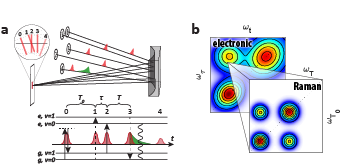
\includegraphics[width=1.0\columnwidth]{Figure1_sci.png}
   \caption{Reprinted and adapted from the original paper\cite{GAMERS}. \textbf{a} The top is a diagram of the 5 separate laser pulses focusing in to the target.  The bottom part of the figure showing pulse the pulses coming in to the system; it also gives a sense for the experimental complexity involved: at minimum, $T_0$, $\tau$ and $T$ all have to be scanned without GRAPES \cite{EngelGRAPES}.  Note the tilt between beams 1 and 2 in the circular inset, which is GRAPES' hallmark.  Also note that the 0th pulse interacts with the system twice, which is why GAMERS is considered a 6-pulse experiment. \textbf{b} An example of the kind of 4-dimensional data they get, showing correlations between energy levels wherever there is signal where the pump(x) frequency is different from the probe(y) frequency.}
	\label{fig:diagram}
\end{figure}


% Graveyard:
% The different forms of absorption spectroscopy are the oldest form of spectroscopy.  Indeed, the first absorption experiment could be said to have taken place in 1802 when Wollaston first noticed odd dark bands in sunlight he had just separated by his improved version of Newton’s prism\cite{Wollaston}.  It turns out the gaps Wollaston observed in the spectrum were molecules between the sun and the experimenter.  Spectroscopy like that eventually proved indispensable to detecting molecules and learning about their structure.  Today there’s not a working scientist whose work doesn’t benefit from absorption spectroscopy whether they directly use it or not.
%
% This process of light interaction provides lots of information about a molecule’s structure through the energy transitions allowed by the method of spectroscopy.  The method can be tuned to tell you more about electrons absorbing energy or the nucleus absorbing energy either through vibrations (Infrared/Raman spectroscopy) or the nuclear spin state through Nuclear Magnetic Resonance (NMR) spectroscopy and its variants.
